% Author: Anachuri Nicolas Daniel
% Template for myself
 
\documentclass[11pt]{article}
\usepackage{indentfirst} 		% First line paragraph indentation
\usepackage{etoolbox} 			% Used for being able to utilise if statements in the language detection.
\setlength{\parskip}{\baselineskip}	% With this line, it is not needed the use of \\ at the end of each paragraph for spacing purposes


% ========================= VARIABLES TO MODIFY =================================

\def\LANGUAGE{EN} %EN, ES		%Language in which the document is going to be written.

\def\reportTile{T. Herramientas Informaticas} 
\def\subject{Trabajo Practico N.1}			%Subject

\def\writter{Anachuri Nicolas Daniel}		%Author(s)


\def\leftUpperHeader{\subject}		%\subject
\def\rightUpperHeader{\leftmark}	%\leftmark for current section


% Do NOT modify anything from here until the beginning of the document.
%============================== DATA PROCESSING ============================
\ifdefstring{\LANGUAGE}{EN}
{

\def\course{1ro del Superior Informatica} %---------
\def\university{Escuela de Minas Dr. Horacio Carrillo} %------------
\def\pageCounterName{PAGE} 		% In the footer will be shown this... 
\def\pageSeparator{OUT OF} 		% ...text in addition of the page number.

}
{
\usepackage[utf8]{inputenc}		%Tildes en caso de no usar arch
\usepackage[spanish, es-tabla]{babel} 	%La opción es-tabla, hace que por defecto las tablas se llamen "Tabla", en vez de "Cuadro".
\def\course{1ro del Superior Informatica} %----------
\def\university{Escuela de Minas Dr. Horacio Carrillo}
\def\pageCounterName{PÁGINA}		%En el pie de página aparece este contenido más el número de página
\def\pageSeparator{DE} 			%DE, OUT OF

}


%===================== USEFUL VARIABLES  =============================
\def\imageSize{0.9}

%===================== PACKAGES TO USE  =============================
\usepackage{amsmath} 			% Allows me the use of matrix in math mode
\setcounter{MaxMatrixCols}{20} 		% Increases the maximum number of columns in matrix from 10 to 20.
\usepackage{pdfpages} 			% Attach pdfs using \includepdf[pages=initial-final]{path.pdf}
\usepackage{lastpage}			% Used to reference the last page and include it in the footer.
\usepackage{xcolor}			% Change color of text and so on. \textcolor{color}{text} is the one I use the most.
\usepackage{placeins} 			% Allows the use of the command \FloatBarrier
\usepackage{setspace}			% Allows the use of the spacing environment to change the space between lines.
\usepackage{graphicx}			% Figures addition
\usepackage{wrapfig}
\usepackage{geometry}			% Changes the geometry of the pages
\usepackage[small, bf]{caption}		% Decreases the size of captions and turns them bold text.
\usepackage{subcaption}			% Include subfigures.
\usepackage{hyperref}			% Allows clickable references.
\hypersetup{colorlinks=true, allcolors=black} 	% Colors of links
\usepackage{pdflscape}			% Allows the use of the environment lscape for landscape pages

\usepackage{fancyhdr}			% Modify header and footer
\usepackage{bm}				% Allows to use bold text in math mode with \bm
\usepackage[makeroom]{cancel}		% Allows the use of \cancelto{}{} to cross out equations
\usepackage{titlesec}			% Change title format
\usepackage{multicol}
\usepackage{hyperref}


%========== CHANGE TITLE FORMAT  ======================
%\titleformat{\section}
%{\bfseries}	% format
%{\thesection}	% label
%{0.3cm}		% separation between label and body
%{}		% code preceding title body
%[]		% code following title body


%========== HEADER AND FOOTER CONFIGURATION ======================
\pagestyle{fancy}
% HEADER[EVEN PAGES]{ODD PAGES}
% Left header
\lhead[
	\scriptsize{\MakeUppercase{\leftUpperHeader}} % Even pages
]
{
	\scriptsize{\MakeUppercase{\leftUpperHeader}} % Odd pages
}

% Central header
\chead[]{}

% Right header
\rhead[
\scriptsize{\rightUpperHeader} % Even pages
]
{
\scriptsize{\rightUpperHeader} % Odd pages
}

\renewcommand{\headrulewidth}{0.8pt}	% Width of the header rule

% FOOTER[EVEN PAGES]{ODD PAGES}
% Left footer
\lfoot[]{}

% Central footer
\cfoot[
\tiny{\pageCounterName\space\thepage\space \pageSeparator\space\pageref{LastPage}} % Even pages
]
{
\tiny{\pageCounterName\space\thepage\space \pageSeparator\space\pageref{LastPage}} % Odd pages
}

% Right footer
\rfoot[]{}
\renewcommand{\footrulewidth}{0.8pt} %Width of the footer rule


%================================== USER OWN FUNCTIONS ===============================================
\newcommand{\PDEA}[1]{\cdot 10^{#1}} % Función para escribir más rápidamente multiplicaciones por potencias de 10. PDEA = Por Diez Elevado A

\usepackage{xargs}	%Permite manejar argumentos opcionales en los comandos creados por el usuario

%Incluir imágenes, la sintaxis es la siguiente:
%\IncludeImage{ruta}[escalado][pie figura][etiqueta], los corchetes son opcionales
\newcommandx*{\IncludeImage}[4][2=1, 3=, 4=]{
	%#1 es la ruta a la imagen
	%#2 es el escalado
	%#3 es el pie de figura
	%#4 es la etiqueta
	
	\begin{figure}[h!]
		\centering
		\includegraphics[width=#2\linewidth]{#1}
		%Si se especifica pie de figura...
		\ifblank{#3}{}{
			\caption{#3}	
		}
		%Si se especifica etiqueta...
		\ifblank{#4}{}{
			\label{#4}	
		}
	\end{figure}
	\FloatBarrier
}


% =============================== MULTI COLUMN CONFIG ==================================

\hypersetup{
    colorlinks=true,
    linkcolor=blue,
    filecolor=magenta,      
    urlcolor=blue,
}

\urlstyle{same}   


%================================ DOCUMENT BEGINNING  =============================================
\begin{document}
%***************** TITLE PAGE (DO NOT MODIFY) ******************************
\begin{titlepage}
	\newgeometry{top=2cm, bottom=3.5cm}

	%Logos Escuela y universidad
	\def\logoSize{0.2}
	\begin{figure}
	\includegraphics[width=\logoSize\linewidth]{/home/nico/Descargas/minas.jpeg}
	\hfill
	\includegraphics[width=\logoSize\linewidth]{/home/nico/Descargas/unju.jpeg}
	\end{figure}


	%Espacio entre logos y título
	\vspace*{1.75cm}

	%Título con interlineado aumentado
	\begin{spacing}{2}
	\centering{
	\Huge{
		\textbf{\reportTile}
	}
	}
	\end{spacing}
	
	%Línea horizontal de la portada
	\hrule
	
	%Se baja al final de la hoja
	\vfill
	\begin{flushright}
	\LARGE{\writter}

	\vspace{2cm}
	
	\Large
	\subject\\
	\course\\
	\university
	
	\vspace{1cm}
	
	\today
	\end{flushright}
	
\end{titlepage}
	
\newgeometry{top=3cm, bottom=3cm}

\tableofcontents
%\cleardoublepage
\clearpage

\begin{multicols}{2}

\section{Actividad 2}

  \subsection{Generaciones de Computadoras}
  
  Puede encontrar la tabla contruida con HTML y CSS \href{https://xo13o.csb.app/}{\underline{aqui}} y el codigo utilizado \href{https://codesandbox.io/s/xo13o}{aqui}
  \begin{wrapfigure}{0.6\linewidth}
  
  \centering
  
\includegraphics[width=0.3\linewidth]{html.png}
  
\includegraphics[width=0.3\linewidth]{css.png}
  \caption{HTML, CSS }
  %\label{fig:etiqueta}
  
  \end{wrapfigure}


  \subsection{Imagenes 1ra Generacion}

  \begin{wrapfigure}{0.6\linewidth}
  
  \centering
  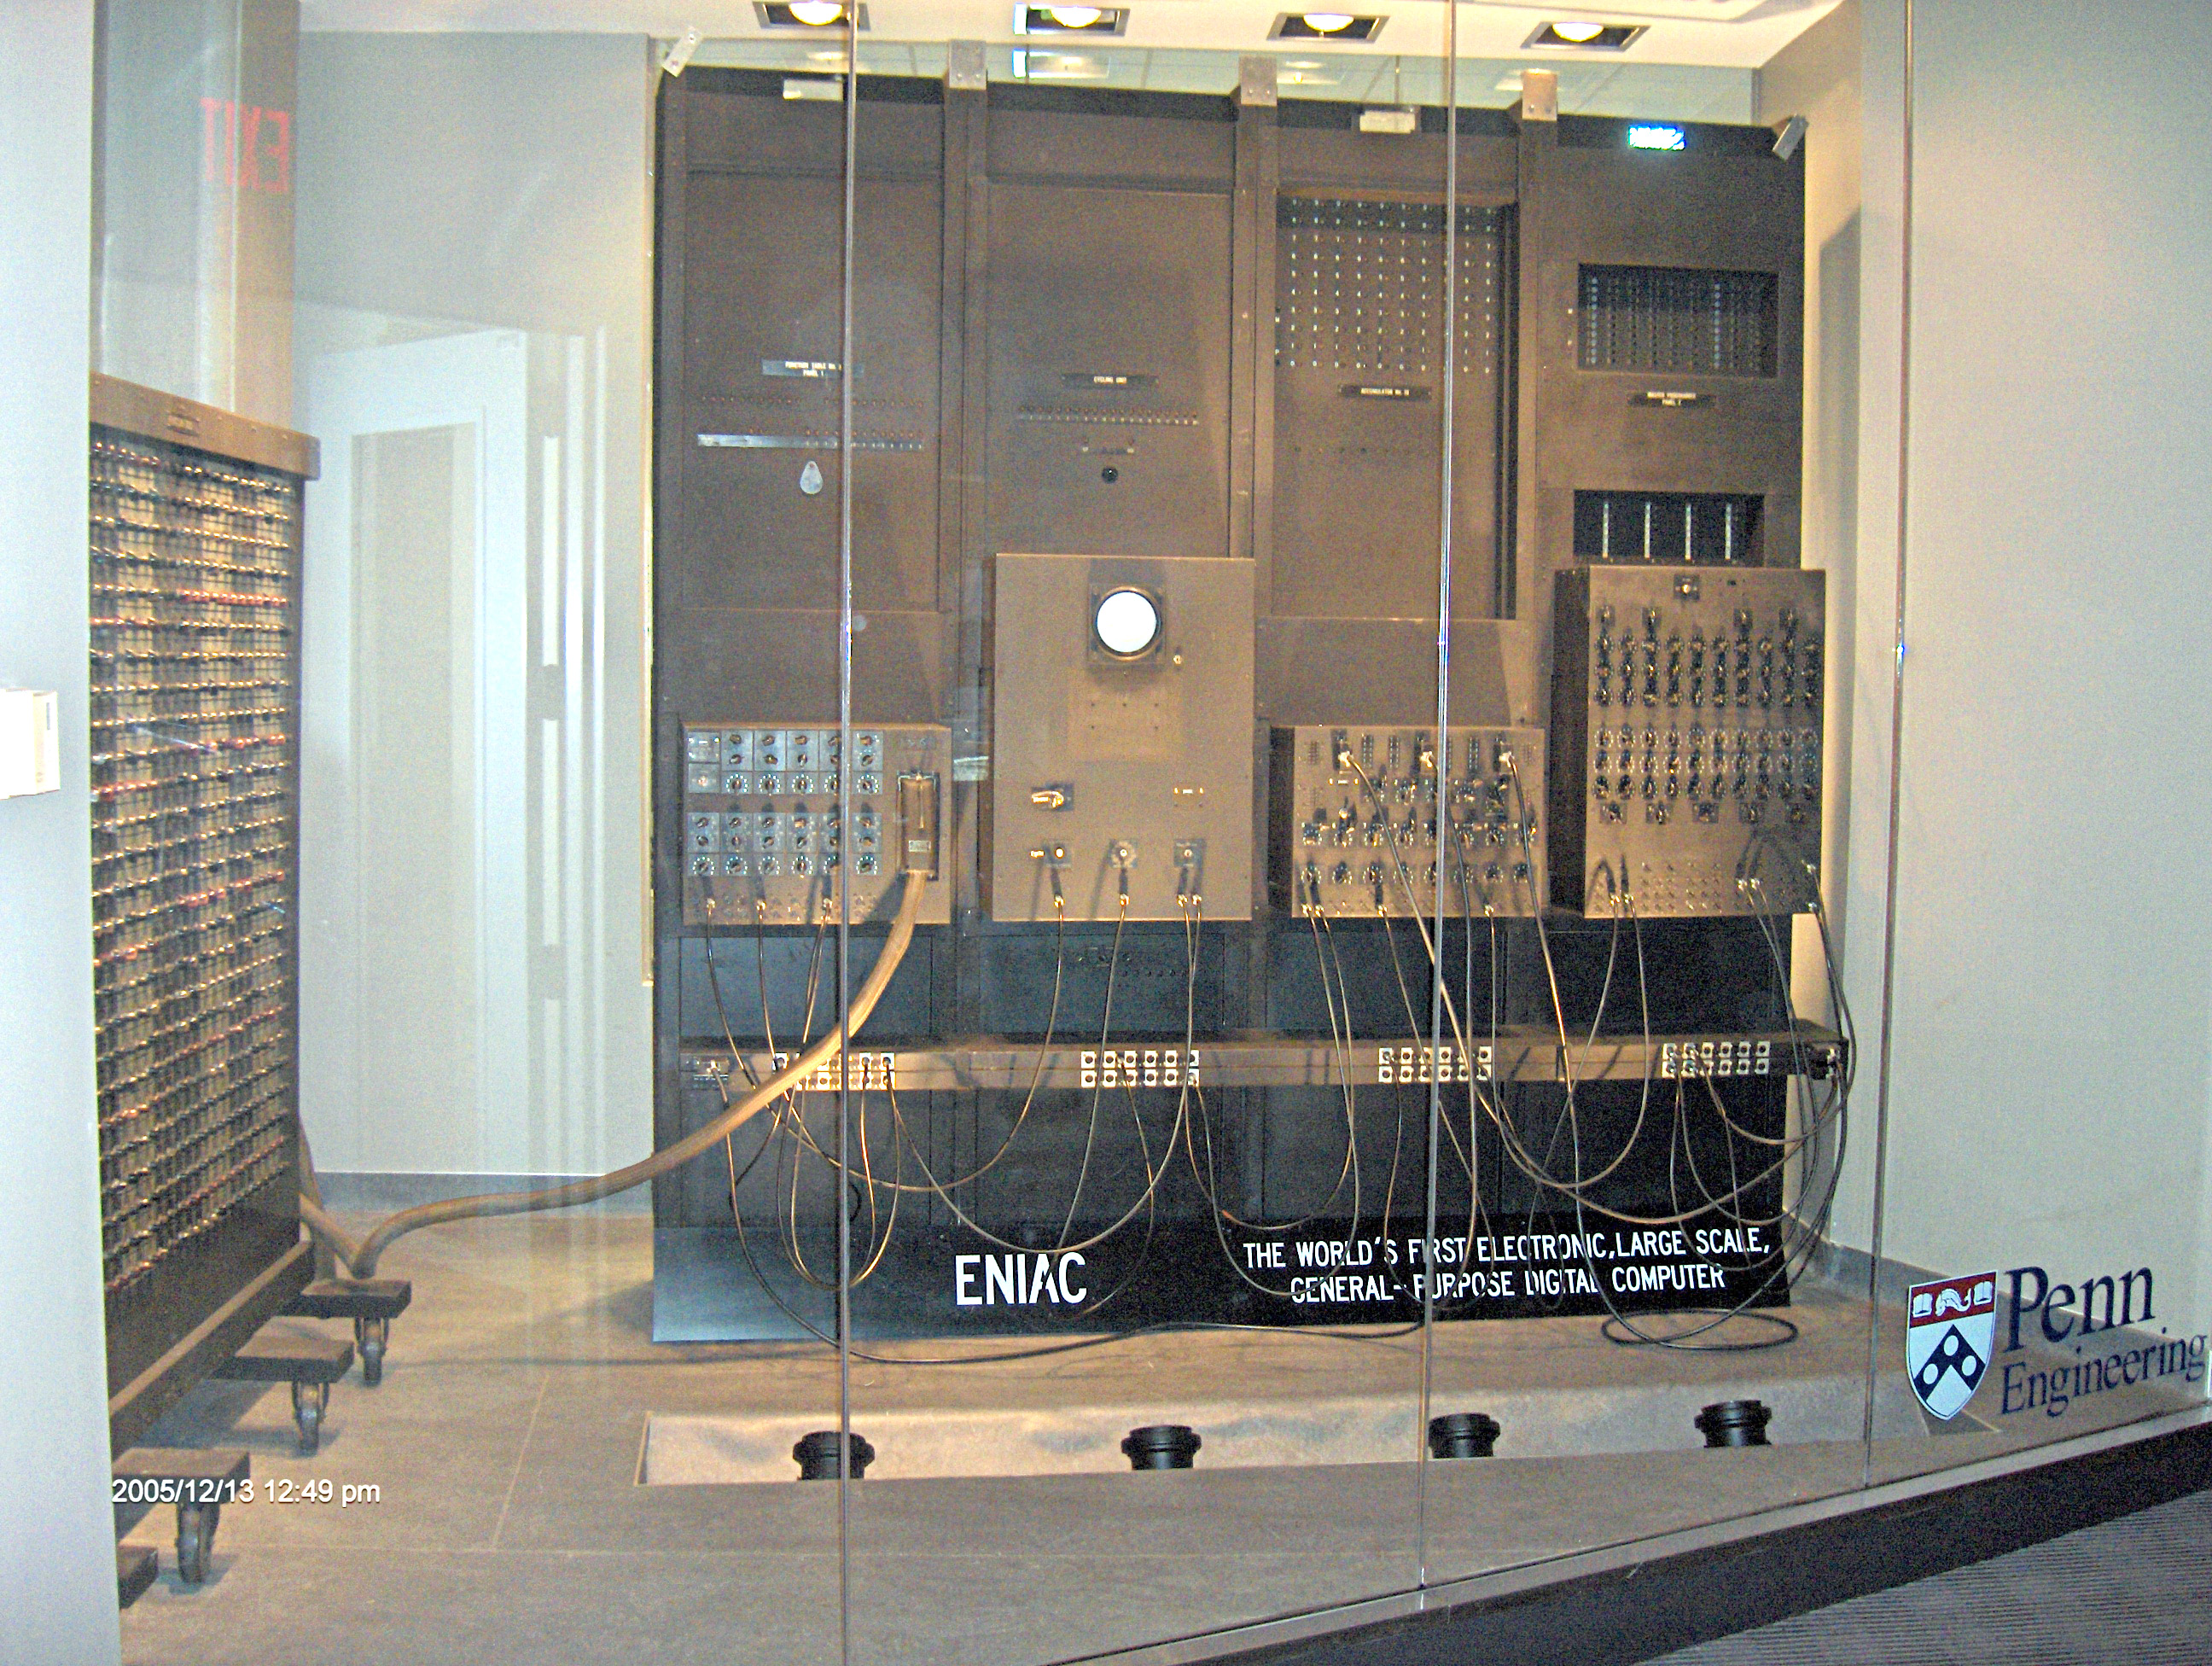
\includegraphics[width=0.3\linewidth]{eniac.jpg}
  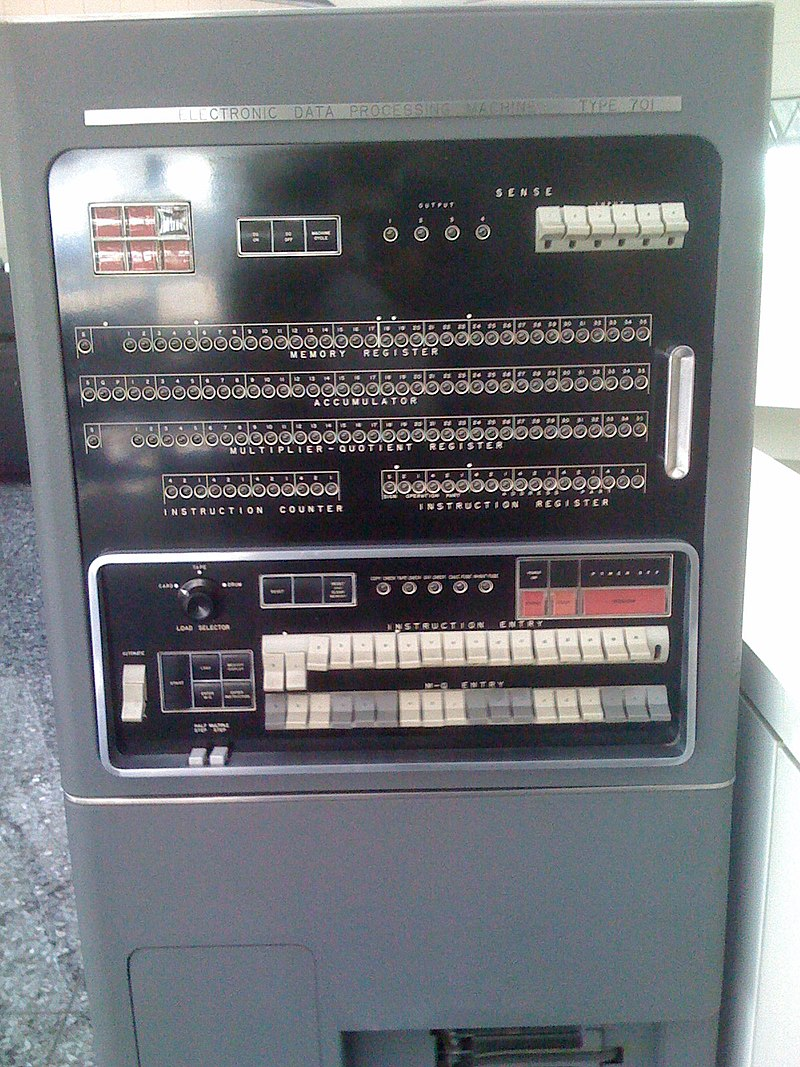
\includegraphics[width=0.3\linewidth]{ibm.jpg}
    \caption{ENIAC (Primera Comutadoras), IBM (International Bussines Machine)}
  %\label{fig:etiqueta}
  
  \end{wrapfigure}

  \subsection{Imagenes 2da Generacion}
  
  \begin{wrapfigure}{0.6\linewidth}
  
  \centering
  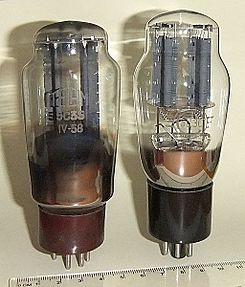
\includegraphics[width=0.3\linewidth]{vacio.jpg}
  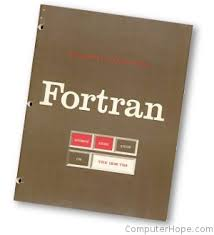
\includegraphics[width=0.3\linewidth]{fortran.jpeg}
  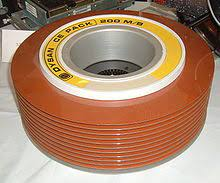
\includegraphics[width=0.3\linewidth]{disco.jpeg}
    \caption{Valculas de Vacio , Fortran primer lenguaje de programacion multi propocito , Disco Magnetico con una capacidad de 5mb}
  %\label{fig:etiqueta}
  
  \end{wrapfigure} 


  \subsection{Imagenes 3ra Generacion}
  
  \begin{wrapfigure}{0.6\linewidth}
  
  \centering
  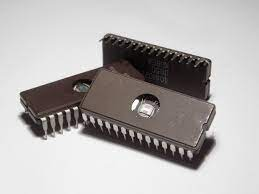
\includegraphics[width=0.3\linewidth]{integrado.jpeg}
  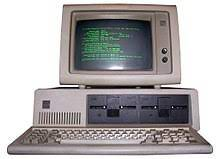
\includegraphics[width=0.3\linewidth]{mini.jpeg}
  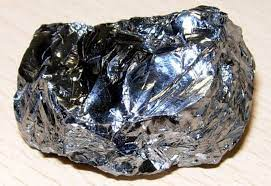
\includegraphics[width=0.3\linewidth]{silicon.jpeg}
  \caption{Circuito Integrado , Minicomptadoras , Silicio utilizaco para la fabricacion de circuitos integrados}
  %\label{fig:etiqueta}
  
  \end{wrapfigure} 

  \subsection{Imagenes 4ta Generacion}
  
  \begin{wrapfigure}{0.6\linewidth}
  
  \centering
  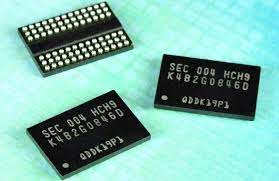
\includegraphics[width=0.3\linewidth]{chip.jpeg}
  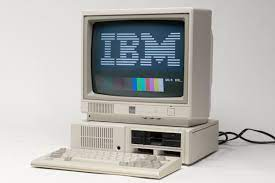
\includegraphics[width=0.3\linewidth]{pc.jpeg}
  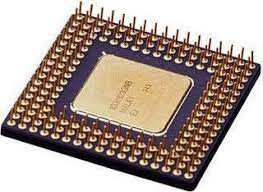
\includegraphics[width=0.3\linewidth]{microprocesor.jpeg}
    \caption{Chip permite controlar procesos de reducida dificultad, PC (Personal Computer ) , Microprocesador}
  %\label{fig:etiqueta}
  
  \end{wrapfigure} 
  
  \subsection{Imagenes 5ta Generacion}

  \begin{wrapfigure}{0.6\linewidth}
  
  \centering
  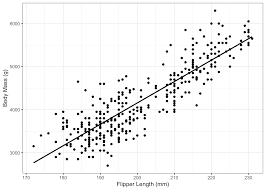
\includegraphics[width=0.6\linewidth]{linear.png}
  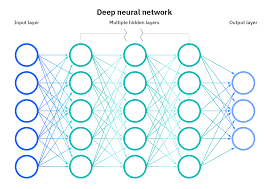
\includegraphics[width=0.6\linewidth]{neural.png}
  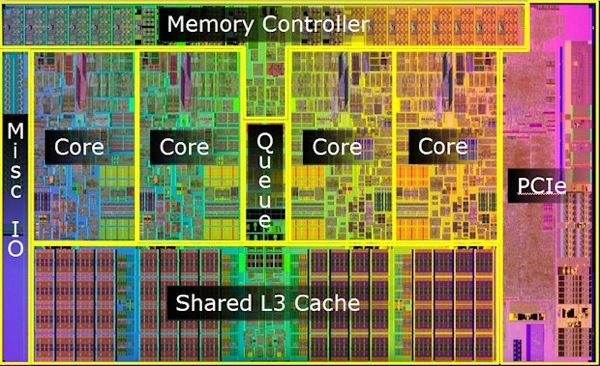
\includegraphics[width=0.6\linewidth]{mcpu.jpg}
    \caption{Grafico de una Regresion Lineal utilizada en el campo del machine Learning (AI), una Red Neuronal Utilizada en Deep Learning (AI), Arquitectura Multi-Cpu de Intel}
  %\label{fig:etiqueta}
  
  \end{wrapfigure} 
  
\section{Actividad 3}
\label{sec:2}

\begin{itemize}
 \item Lea el documento del aula virtual: resuma en forma cronológica por cada año que aparezca en el mismo

  \begin{itemize}
      
    \item 1920:  Primera transmicion publica de radio.
      
    \item 1930:  Comptadoras Electromecanicas
      
    \subsection{Primera Generacion}
    \item 1947: \textbf{ENIAC} Primera computadora digital electronica.
    \item 1949: \textbf{EDVAC} Primera computadora programable.
    \item 1951: \textbf{UNIVAC} Primerda computadora comercial. 
    \item 1953: \textbf{IBM 701} Primera computadora de IBM  (Intenational Bussniness Machine)
    \item 1954: Introduccion de una nueva forma de almacenamiento de datos (Tambor Magnetico)
    \subsection{Segunda Generacion}
    \item 1959: Uso de Transitores en computadoras 
    \item 1962: Nacen los primeros programas con interfaces visuales (UI)  
    \item Desarrollo de varios lenguajes de programacion 
    \subsection{Tercera Generacion: Circuitos Integrados}
    
    \item 1964: Nacimiento de los Circuitos integrados

    \item Medios Magniticos de Almacenamiento 
    \item \textbf{IBM 360}
    
    \subsection{Cuarta Generacion: Microprocesadores , "Miniaturizacion"}
    
    \item remplazar nucleos magneticos con chips de silicio
    
    \item 1971: Se presenta en primer microprocesador
      
    \item 1977: Primeras Microcomputadoras (Computadoras de escritorio)
    
    \subsection{Quinta Generacion: Inteligencia Artificial}
    \item 1982: Presentacion de la primera supercomputadora  
    
    \item Robotica
    
    \subsection{Sexta Generacion}

    \item Arquitecturas paralelo vectorial
      
    \item Redes de Area mundial
    \item 
  \end{itemize}
  
  
\subsection{¿En la actualidad, cuales serían las características de una PC y a que precio de mercado conseguiría la misma?Compare las características a ésa fecha.}

La evolución de las características ha sido exponencial y realmente seria absurdo tratar de enfrentar un PC del siglo XX con las del XXI. Antes de verlas debemos de estar consientes de cuáles son sus componentes \textbf{principales} de una PC. 
\begin{itemize}
  \item \textbf{CPU} (Central Procesor Unity)  componente principal de un ordenador engargado de todos los procesos llevados acabo. Sus caracteristicas actuales son:
  \begin{itemize}
    \item Modelo intel i9 9900k
    \item Nucleos: 8 
    \item Frequencia:  3.60 GHz
    \item cache:  16 MB
    \item Consumo: 95 W
    \item precio: 46.000 
  \end{itemize}

  \item \textbf{GPU} (Graphics Procesor Unity)  componente encargado de realizar calculos vectoriales y matriciales.
    
  \begin{itemize}
    \item Modelo: RTX 3090
    \item Velocidad de Reloj: 1.7GHz.
    \item Memoria: 24GB GDDR6X.
    \item Tipo de Memoria: GDDR6X.
    \item Precio: 40.000 
  \end{itemize}
  
  \item \textbf{Memoria Ram} encargado de enviar informacion de forma rapida cuando la CPU la necesite
  
  \begin{itemize}
    \item Modelo: Team Xtreem ARGB DDR4-3600 C14 gaming memory review
    \item Tipo de Memoria: DDR4  
    \item Capacidad 16GB
    \item velocidad 3,600MHz
    \item voltage: 1.45v
    \item Precio: 9000 
  \end{itemize}
    
  \item \textbf{Almacenamiento} guarda toda la informacion del sistema y del usario.
  
  \item Modelo: Samsung 850 EVO M.2 
  \item Capacidad: 120GB, 250GB, 500GB.
  \item Tipo: SSD
  \item Precio: 20.000 
  
    
\end{itemize}

Los Precios fueron listados desde MercadoLibre Argentina con precio total de 115.000 pesos argentinos.




\end{multicols}

\end{document}

